\chapter{État de finalisation du projet}

\paragraph{}
En cette fin de projet, nous sommes en capacité de fournir une application fonctionnelle qui remplit les exigences principales du cahier des charges. Nous expliquerons en détail les différentes fonctionnalités implémentées, pour le serveur puis pour le client. Pour mettre en lumière les différences avec le projet tel que nous l'avions imaginé au moment de la conception, cette partie du rapport peut être considérée comme un second rapport de conception, plus bref cette fois-ci, car les éléments qui sont restés identiques à ce premier rapport de conception ne seront pas détaillés. Au besoin, nous introduirons des éléments techniques, facilement compréhensibles pour un lecteur ayant déjà programmé en Java.

\section{Architecture générale et technologies utilisées}

\paragraph{}
Concernant les technologies, le rapport de conception comportait déjà tous les éléments utilisés. La seule différence est le reconnaisseur d'écriture manuscrite. En effet, par manque de temps, nous n'avons pas pu mettre en place de connexion effective avec un reconnaisseur d'écriture manuscrite. Le reconnaisseur Laia, mentionné dans le rapport de conception, n'est donc pas présent dans le projet, cette partie étant optionnelle dans le cahier des charges initial du projet, qui consiste à principalement générer les bases d'apprentissage. Nous avons donc utilisé SQLite pour la base de données, OpenCV pour la découpe d'images, Angular 7 pour l'interface client, Grizzly pour le serveur web, ainsi que Jersey pour l'API REST. L'architecture du serveur est sensiblement la même, car nous avons souhaité continuer sur le modèle d'un contrôleur qui orchestre toute l'application, découpée en modules : préparation des données, connexion avec la base de données, interface avec le reconnaisseur.

\section{Côté serveur}

\paragraph{}
Du côté du serveur, nous avons développé une application principale en Scala, ainsi que quelques scripts en Python pour le prétraitement des données XML et le traitement d'images, que nous présenterons également. La différence principale avec le rapport de conception est la présence de ces scripts. Nous avions en effet prévu dans un premier temps de fournir une application serveur monolithique, développée en un seul langage de bout en bout. L'expérience nous a montré qu'il était plus judicieux d'utiliser des scripts comme outils venant appuyer cette application. Nous détaillerons, paquetage par paquetage, le contenu technique et son utilité pour le projet.

\subsection{Application en Scala}

\paragraph{}
L'application principale se construit autour de deux paquetages en plus de l'objet \texttt{Main} qui lance le serveur web :
\begin{itemize}
\item un premier paquetage \texttt{model} qui contient tous les éléments utiles du serveur, \textit{i.e.} des outils pour traiter les données d'entrée, les images, créer les exemples, et interagir avec la base de données et les reconnaisseurs d'écriture manuscrite ;
\item un paquetage \texttt{resource} qui contient une classe permettant de recevoir les appels REST du client, d'appeler les bonnes méthodes dans les classes du paquetage précédent, et de façonner les réponses HTTP qui contiennent les résultats de ces méthodes.
\end{itemize}
Détaillons à présent le paquetage \texttt{model}. Celui-ci est composé de plusieurs sous-paquetages : \texttt{common}, \texttt{database}, \texttt{preparation}, et \texttt{recogniser}.

\begin{mdframed}[frametitle={Figure 1 : Paquetage \texttt{common}}, innerbottommargin=10]
\begin{center}
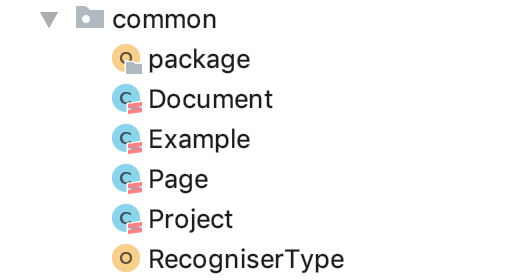
\includegraphics[scale=0.7]{assets/common.png}
\end{center}
\end{mdframed}

\paragraph{}
Le paquetage \texttt{common} présenté en Figure 1 contient les classes qui correspondent aux éléments stockés en base de données : des projets contenant des documents composés de pages, ces pages contenant après traitement des exemples d'apprentissage pour les reconnaisseurs d'écriture manuscrite. Le \textit{package object} est une particularité de Scala. Il s'agit d'un objet associé au paquetage, qui contient des définitions utilisées dans le paquetage ainsi qu'en dehors, sémantiquement dépendantes de ce paquetage, mais n'appartenant pas à une classe en particulier. Une valeur \texttt{value} pourra être appelée avec \texttt{common.value}. Dans ce cas, le \textit{package object} contient des chemins vers différents dossiers ou exécutables sur le système de fichiers, notamment l'endroit où sont stockés les fichiers images ainsi que les exportations d'exemples, ou les scripts de traitement d'images.

\begin{mdframed}[frametitle={Figure 2 : Paquetage \texttt{database}}, innerbottommargin=10]
\begin{center}
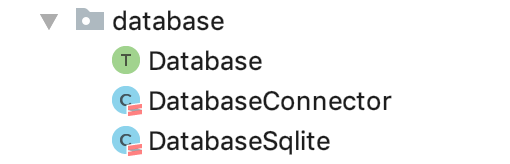
\includegraphics[scale=0.7]{assets/database.png}
\end{center}
\end{mdframed}

\paragraph{}
Le paquetage \texttt{database} contient les classes qui permettent au logiciel de faire des requêtes sur la base de données associée au serveur, qui contient les différents exemples qui seront fournis aux reconnaisseurs d'écriture manuscrite. Le \textit{trait} \texttt{Database} (un \textit{trait} en Scala est l'équivalent d'une interface en Java) décrit toutes les actions que l'on doit pouvoir effectuer depuis l'extérieur sur la base de données, et la classe \texttt{DatabaseSqlite} l'implémente pour le SGBD SQLite que nous avons choisi pour ce projet. L'utilisation d'un \textit{trait} permet à un développeur réutilisant le projet de changer le SGBD du serveur au besoin. Par exemple, pour un passage réel en production, une base de données MySQL peut être un choix judicieux. 

\paragraph{}
La classe \texttt{DatabaseConnector} vient d'un concept que nous avons décidé de suivre tout au long du projet du côté du serveur. Pour chaque paquetage du serveur, le connecteur reçoit les différents appels de l'extérieur, et les relaie vers l'implémentation choisie du \textit{trait} concerné par ce paquetage. Cela permet de choisir localement l'implémentation en changeant une ligne dans un fichier.

\begin{mdframed}[frametitle={Figure 3 : Paquetage \texttt{preparation}}, innerbottommargin=10]
\begin{center}
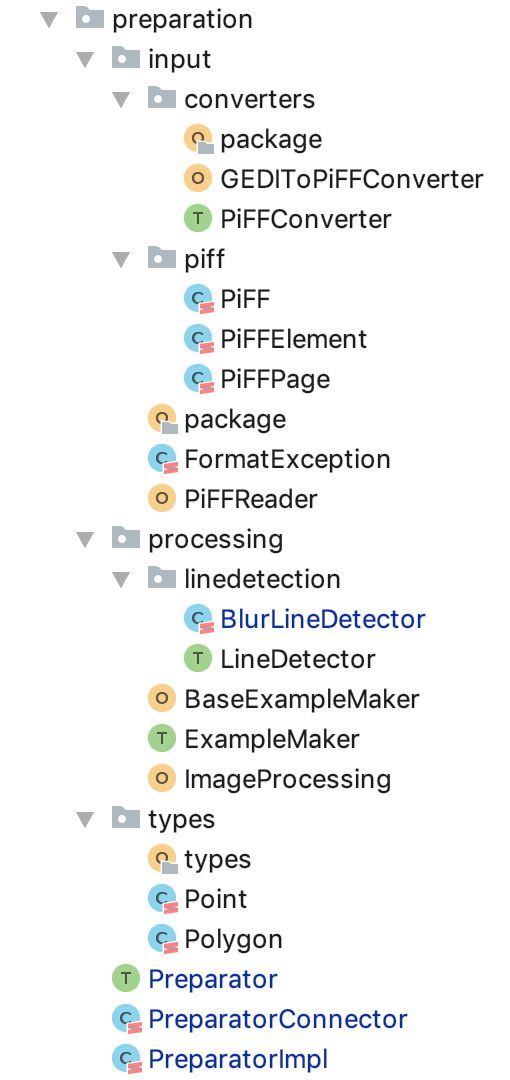
\includegraphics[scale=0.7]{assets/preparation.png}
\end{center}
\end{mdframed}

\paragraph{}
Le paquetage \texttt{preparation} est assez complexe. Il est en trois parties : un sous-paquetage \texttt{input} qui gère la lecture des données d'entrée, un sous-paquetage \texttt{processing} qui réalise le traitement d'images et la création d'exemples, et un sous-paquetage \texttt{types} qui contient des définitions d'objets géométriques tels que les points ou les polygones, utiles pour les autres classes du paquetage.

\paragraph{}
Le sous-paquetage \texttt{input} contient la définition du format PiFF, format principal manipulé par notre logiciel. Il contient également un \textit{trait} définissant un convertisseur d'un format quelconque vers PiFF ainsi qu'une implémentation de ce dernier pour traiter le format GEDI dans lequel sont écrites toutes les vérités terrain de la base Maurdor, base d'apprentissage à laquelle nous avons eu accès tout au long du projet. Enfin, il contient un objet \texttt{PiFFReader} permettant de lire une vérité terrain dans les formats PiFF (ou GEDI à l'aide des convertisseurs) à partir d'un fichier, et d'en faire un objet \texttt{PiFF} manipulable par toutes les autres parties de notre logiciel.

\paragraph{}
Le sous-paquetage \texttt{processing} a quant à lui pour \textit{trait} principal \texttt{ExampleMaker}, qui définit un créateur d'exemples à partir d'un objet \texttt{PiFF}. Il en contient une implémentation, \texttt{BaseExampleMaker}. Ces créateurs d'exemples se basent sur l'objet \texttt{ImageProcessing} pour toutes leurs découpes d'images. La découpe est réalisée avec un script Python qui sera présentée plus tard dans ce rapport. Un sous-paquetage \texttt{linedetector} est présent. Il s'agit d'un détecteur de lignes fourni par l'encadrant de projet, qui permet de découper les images de manière plus efficace. En effet, la première découpe peut donner des paragraphes, or le reconnaisseur ne s'entraîne que sur des lignes. Il est donc plus pertinent de faire une seconde découpe pour s'assurer que nous obtenons bien des lignes en sortie.

\paragraph{}
Enfin, ce paquetage \texttt{preparation} contient un \textit{trait} \texttt{Preparator}, qui définit un objet qui crée des exemples à partir d'une page d'un document et de sa vérité terrain. Comme pour le paquetage précédent, nous fournissons également une implémentation du \textit{trait} ainsi qu'un connecteur.

\begin{mdframed}[frametitle={Figure 4 : Paquetage \texttt{recogniser}}, innerbottommargin=10]
\begin{center}
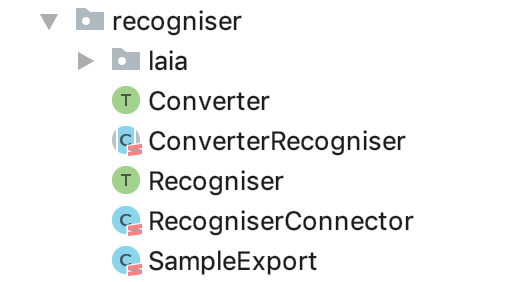
\includegraphics[scale=0.7]{assets/recogniser.png}
\end{center}
\end{mdframed}

\paragraph{Reconnaisseur}
Dans la première vision de l'interface avec le reconnaisseur que nous avions, nous souhaitions intégrer celui-ci à notre application. C'est-à-dire, pourvoir effectuer depuis celle-ci son entrainement, son évaluation ainsi que son utilisation pour reconnaître des imagettes. Cependant, nous avons dû réduire ces fonctionnalités afin de permettre une meilleure souplesse à l'utilisateur. En effet, celui-ci n'est plus obligé de brancher son reconnaisseur au logiciel afin que celui-ci puisse utiliser la base de connaissance. Cette modification de point de vue nous a également permit de gagner du temps vis-à-vis de cette partie. Ainsi, nous n'avons plus qu'une fonction \textit{export} permettant l'exportation des exemples générés dans le format du reconnaisseur avec les fichiers nécessaires afin d'en faciliter l'utilisation.
Nous avons fourni une exportation par défaut qui permet d'obtenir l'image de l'exemple ansi qu'un fichier texte contenant sa transcription. Ces deux fichiers étant nommés de la même manière afin de pouvoir les associer facilement.
Cependant, il n'est pas certain que dans le temps restant l'implémentation de l'exportation pour le reconnaisseur de Laia soit opérationnel comme il était prévu à l'origine.

Le paquetage \texttt{recogniser} est constitué de deux \textit{trait} qui prennent en charge deux aspect de l'exportation. Le \texttt{Converter} permet de contraindre les images de la base au format d'entrée du reconnaisseur selectionné tandis que le \texttt{Recogniser} se charge de la création des fichiers nécessaires à l'apprentissage du reconnaisseur à partir de la base. Afin de lier ces deux parties, la classe abstraite \texttt{ConverterRecogniser} est utilisée. C'est donc de celle-ci qu'héritent les classes de conversions qui sont à implémenter. Nous fournissons alors les classes \texttt{SampleExport} qui est la classe d'export par défaut qui ne formatte donc rien et ne délivre que les images et leur transcription de la facon expliquée précédemment, ainsi qu'une classe \texttt{LaiaRecogniser} qui permettra d'exporter pour le reconnaisseur Laia avec les fichiers nécessaires (il n'est cependant pas sur que cette partie soit complètement implémentée dans le temps restant).
Ce paquetage possède également un connecteur comme les autres afin de le lier au \texttt{Controller}.

\paragraph{Controleur}
Enfin, ce paquetage \texttt{model} contient une classe \texttt{Controller} avec toutes les méthodes du modèle utilisées par la ressource REST, ainsi qu'une classe \texttt{ImplFactory} donnant toutes les implémentations choisies des différents \textit{traits} dans chaque sous-paquetage.

\subsection{Scripts Python}

\paragraph{}
Pour appuyer l'application serveur en Scala, nous avons développé trois scripts en Python. Le premier, \texttt{tiffsplitter.py}, permet de découper à l'aide d'\href{https://opencv.org/}{OpenCV} une image TIFF multipages en plusieurs images TIFF avec une seule page chacune. Le second, \texttt{gedisplitter.py}, permet de couper un fichier de vérité terrain dans le format GEDI en plusieurs fichiers GEDI, chacun faisant référence à une seule image, donc une seule page. Ce script utilise la bibliothèque \href{https://pypi.org/project/defusedxml/}{defusedxml} car l'outil de manipulation des fichiers XML présent dans la bibliothèque standard de Python présente d'après leur site Internet des vulnérabilités logicielles. Ces deux premiers scripts permettent d'avoir des données d'entrée qui correspondent à un couple image - vérité terrain pour une page de texte manuscrit. Le dernier script, \texttt{imagecropper}, réalisé aussi avec OpenCV, permet de réaliser les découpes d'images à partir d'une zone rectangulaire donnée en argument.

\section{Côté client}
\paragraph{}
Notre IHM contient trois pages : une page d'accueil, une page d'annotation manuelle et une page de validation des transcriptions. Nous avions initialement prévu d'inclure également une page de découpe manuelle des zones du manuscrit, mais nous nous sommes trouvés dans l'incapacité de la réaliser par manque de temps.

\paragraph{}
Nous avons réalisé notre interface en \texttt{TypeScript}, \texttt{Angular} et \texttt{HTML}. Elle compte quatorze composants en tout :
\begin{itemize}
\item trois composants principaux, soit un pour chaque page de l'interface (accueil, annotation et validation);
\item dix composants dédiés aux différentes fenêtres de \textit{dialog} qui apparaissent au fil de l'interface. Ce sont des fenêtres qui se superposent à la page de l'interface pour remplir des tâches très précises, comme configurer un nouveau projet, afficher des instructions sur le fonctionnement de l'interface ou encore demander une indication à l'utilisateur ;
\item un dernier composant \texttt{service} qui se charge d'effectuer certains appels à la ressource REST pour alléger le code des composants des pages principales.
\end{itemize}

\begin{mdframed}[frametitle={Figure 5 : Arborescence des composants de l'interface}, innerbottommargin=10]
\begin{center}
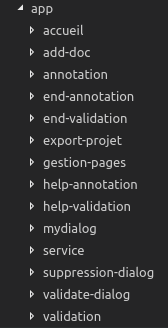
\includegraphics[scale=0.5]{assets/arborescenceIHM.png}
\end{center}
\end{mdframed}

\paragraph{}
Chaque page de l'interface est dédiée à une fonctionnalité. La page d'accueil permet de naviguer dans les projets et les documents afin de choisir le manuscrit à annoter. Elle propose également de créer de nouveaux projets en choisissant le nom du projet, le reconnaisseur associé, les documents qui le composent et les pages des documents. L'utilisateur peut également supprimer des documents faisant partie d'un projet ou encore des projets entiers.

\paragraph{}
Sur la page d'annotation manuelle, l'utilisateur peut visualiser le manuscrit découpé ligne par ligne ainsi que la transcription associée sous chaque imagette. Il peut modifier cette transcription en la tapant au clavier. Si un exemple (un couple imagette-transcription) semble manquer de pertinence, l'utilisateur peut le cacher à l'aide d'une croix cliquable située dans le coin supérieur droit de l'imagette. L'exemple est alors grisé sur l'interface et il n'est pas pris en compte lors de l'export des données vers le reconnaisseur du projet. L'utilisateur a encore à tout moment la possibilité de réhabiliter l'exemple en cliquant sur la flèche qui a remplacé la croix en haut à droite de l'imagette.

\paragraph{}
Enfin, la page de validation permet une relecture rapide des transcriptions pour effectuer une validation finale. L'utilisateur peut également cacher un exemple qui manque de pertinence, comme sur la page d'annotation. Un simple appui sur \texttt{Entrée} permet de valider d'un seul coup toutes les transcriptions affichées sur la page courante.

\paragraph{}
Nous avons développé l'ergonomie de notre application autant que possible dans le temps restreint dont nous disposions et nous avons tenté de fournir une application aussi intuitive que possible en facilitant son utilisation et en simplifiant les gestes requis par l'utilisateur (minimum de mouvements de souris, raccourcis clavier...). Cependant, l'ergonomie n'est pas optimale et nécessiterait des améliorations, notemment au niveau de la répétition de certains gestes par l'utilisateur qui requièrent de la précision. Toutefois, nous avons préféré mettre l'accent sur la stabilité et le bon fonctionnement de notre application avant de dédier le temps restant à l'amélioration de l'ergonomie.
